\documentclass{beamer}
\usetheme{Nord}
\usepackage{tikz}
\usetikzlibrary{automata,positioning}
\usepackage{array}
\usepackage{booktabs}
\usepackage{amsmath}

% Remove date and modify title page
\title{Finite State Automata}
\author{}
\date{}

% Remove navigation symbols
% \setbeamertemplate{navigation symbols}{}

% Remove "on" from title page
\makeatletter
\setbeamertemplate{title page}{
  \vbox{}
  \vfill
  \begingroup
    \centering
    \begin{beamercolorbox}[sep=8pt,center]{title}
      \usebeamerfont{title}\inserttitle\par%
      \vskip0.25em%
    \end{beamercolorbox}%
    \vskip1em\par
    \begin{beamercolorbox}[sep=8pt,center]{author}
      \usebeamerfont{author}\insertauthor%
    \end{beamercolorbox}
  \endgroup
  \vfill
}
\makeatother

\begin{document}

\begin{frame}
    \titlepage
\end{frame}

% Table of Contents slide
\begin{frame}
    \frametitle{Contents}
    \tableofcontents[currentsection]
\end{frame}

% Section 1
\section{Introduction}
\begin{frame}
    \frametitle{What is Finite State Automata?}
    % Simple bullet points
    \begin{itemize}
        \item A Finite State Automata (FSA), also known as a Finite State Machine (FSM), is a mathematical model used to represent and control the execution of processes that can be in a finite number of states
        \item Imagine it as a simple computer with a limited amount of memory. It can only be in one state at a time and transitions between these states based on the input it receives.
        \end{itemize}
\end{frame}

% Section 2
\section{Definition}
\begin{frame}
    \frametitle{Definition}
    % Block environment
    \begin{block}{Definition}
        Finite state automata is 3 tuple(S, \Sigma,T) where 
        
        \begin{itemize}
            \item[\( S \)] A finite set of states, one of which is the initial state $s_{init}$.
            \item[\( \Sigma \)] The alphabet, of source symbols.
            \item[\( T \)] is a finite set of state transitions defining transitions out of each $s_i $ \epsilon \ S on encountering the symbols \Sigma.
        \end{itemize}

    \end{block}
    
\end{frame}

\begin{frame}
    \frametitle{State Transitiion Tables}
    \begin{itemize}
        \item We label the transitions of FSA using the conventions:\\
            A transition out of $s_i$ \epsilon\ S on encountering a symbol symb \epsilon \ \Sigma\ has the label symb
        \item We say a symbol symb is recognized by FSA when the FSA makes a transition labelled symb.
        \item The transitions in an FSA can be represented in the form of a State Transition Table (STT).
        \item An STT has one row for each state $s_i$ and one column for each symbol symb \epsilon\ \Sigma\
    \end{itemize}
\end{frame}

\begin{frame}
    \frametitle{State Transition Tables Contd}
    \begin{itemize}
        \item An entry in STT($s_i$, symb) in the table indicates the id of the new state entered by the FSA if there exists a transition labelled symb in state $s_i$.
        \item if the FSA does not contain a transition out of state $s_i$ we leave STT($s_i$, symb) blank    
        \item A state transition can also be represented by a triple (old state, source symbol, new state).
        \item thus the entry STT($s_i$, symb) = $s_j$ and the triple ($s_i$, symb, $s_j$) are equivalent.

    \end{itemize}
\end{frame}
% Frame with columns
\section{Types}
\begin{frame}
    \frametitle{Types}
    \begin{itemize}
        \item Deterministic FSA
        \item Non Deterministic FSA
    \end{itemize}
\end{frame}


\begin{frame}
    \frametitle{Deterministic FSA}

    \begin{itemize}
        \item In DFA Transitions are Deterministic , that is at most one transition exists in state $s_i$ for a symbol symb
        \item[\( Defintion \)] A deterministic finite state automation (DFA) is an FSA such that $t_i$ \epsilon \ T, $t_1$ \equiv\ ($s_i$, symb, $s_j$) 
        \newline implies \ni! \ $t_2$ \epsilon \ T, $t_2$ \equiv\ ($s_i$, symb, $s_k$)
    \end{itemize}
    
\end{frame}
% Section 4
\section{Deterministic FSA}
\begin{frame}
    \frametitle{Deterministic FSA}

    \begin{itemize}
        \item At any point in time DFA would recognize some prefix \alpha \ of the source string, possibly the null string.
        \item The operation of DFA is history sensitive because its current state is a function of the prefix recognized by it.
        \item The DFA halts when all symbols in the source string are recognized, or an error condition is encountered.
        \item The string is valid if and only if the DFA recognizes every symbol in the string and find itself in a final state at the end of the sring.
            

    \end{itemize}
\end{frame}

\begin{frame}
    \frametitle{Transition Table}
    \begin{table}
        \centering
        \begin{tabular}{c|cc}
            \toprule
            State & \multicolumn{1}{c}{Next Symbol} \\
            & d  \\
            \midrule
            Start & Int &  \\
            Int & Int &  \\
            \bottomrule
        \end{tabular}
        \caption{STT to recognize integer string}
    \end{table}
\end{frame}



% Frame with a figure
\begin{frame}
    \frametitle{Visual Representation}
   % Example of a complex DFA that accepts strings ending with 'abb'
\begin{figure}
    \centering
    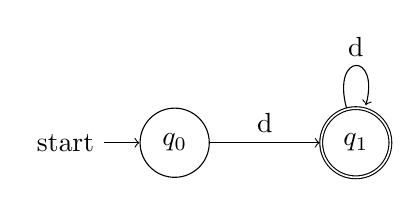
\begin{tikzpicture}[auto, node distance=2.3cm, scale=1]
        % Define states
        \node[state,initial] (Start) {$q_0$};
        \node[state,accepting] (Int) [right of=Start] {$q_1$};
      
        \path[->]
        % For identifies (starting with letter/underscore)
        (Start) edge node {d} (Int)
        (Int) edge[loop above] node {d} (Int);
        
        
        
    \end{tikzpicture}
    \caption{DFA for Integer strings}
\end{figure}
\end{frame}

\begin{frame}
    \frametitle{DFA States Description}
    \begin{description}
        \item[$q_0$] Initial state
        \item[$q_1$] Valid identifier state (accepts only integer strings)
        % \item[$q_5$] Final decimal number state
    \end{description}
    
    Accepts:
    \begin{itemize}
        \item Literals: 42, 314, 1234 100
    \end{itemize}
\end{frame}

% Section 5
\section{Regular Expressions}

\begin{frame}
    \frametitle{Regular Expressions}
    \begin{itemize}
        \item[\( Definition \)] Regular expressions are a generalization of type 3 production rules.
        \item The regular expression generalizes on Type 3 rules by premitting multiple occurences of a string form, and concatenation of strings.

    \end{itemize}
\end{frame}

\begin{frame}
    \frametitle{Some Regexes}

     \begin{table}[h]
        \centering
        \begin{tabular}{c|c} 
            \hline
            Regular Expression & Meaning \\ 
            \hline
            \( r \) & string \( r \) \\
            \( s \) & string \( s \) \\
            \( r.s \) or \( rs \) & concatenation of \( r \) and \( s \) \\
            \( (r) \) & same meaning as \( r \) \\
            \( r \,\vert\, s \) or \( (r \,\vert\, s) \) & alternation, i.e., string \( r \) or string \( s \) \\
            \( (r) \,\vert\, (s) \) & alternation \\
            \( [r] \) & an optional occurrence of string \( r \) \\
            \( (r)^{*} \) & 0  or more occurrences of string \( r \) \\
            \( (r)^{+} \) &  1  or more occurrences of string \( r \) \\
            \hline
        \end{tabular}
        \caption{Regular Expression Notation}
    \end{table}
\end{frame}

% Section 6
\section{Building A DFA}

\begin{frame}
    \frametitle{DFA for integers, real numbers and identifiers}
   % Example of a complex DFA that accepts strings ending with 'abb'
\begin{figure}
    \centering
    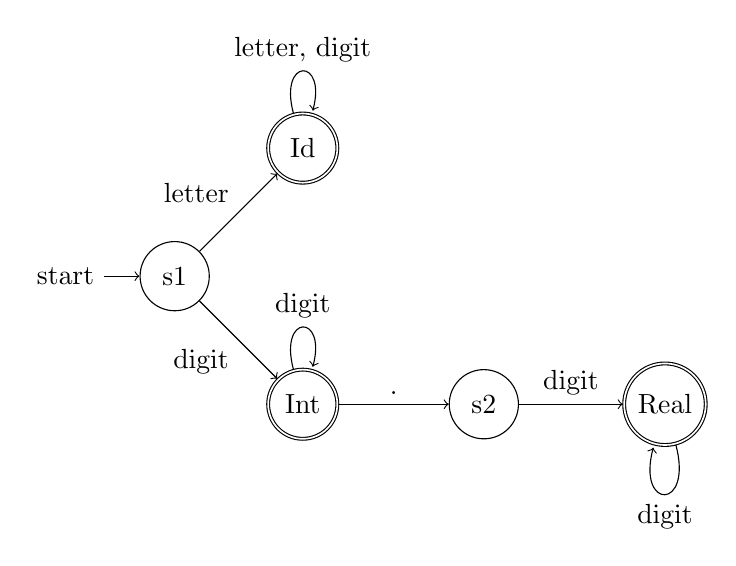
\begin{tikzpicture}[auto, node distance=2.3cm, scale=1]
        % Define states
        \node[state,initial] (Start) {s1};
        \node[state,accepting] (Id) [ above right of=Start] {Id};
        \node[state,accepting] (Int) [below right of=Start] {Int};
        \node[state] (s2) [right of=Int] {s2};
        \node[state,accepting] (Real) [right of=s2] {Real};
        % \node[state,accepting] (q5) [right of=q4] {$q_5$};
        
        % Define transitions
        \path[->]
        % For identifiers (starting with letter/underscore)
        (Start) edge node {letter} (Id)
        (Id) edge[loop above] node {letter, digit} (Id)
        
        % For numeric literals
        (Start) edge node[swap] {digit} (Int)
        (Int) edge[loop above] node {digit} (Int)
        (Int) edge node {.} (s2)
        (s2) edge node {digit} (Real)
        % (q4) edge node {digit} (q5)
        (Real) edge[loop below] node {digit} (Real);
        % (q5) edge[loop below] node {digit} (q5);
        
    \end{tikzpicture}
    \caption{DFA for Identifiers and Numeric Literals}
\end{figure}
\end{frame}
% Add Legend/Description
\begin{frame}
    \frametitle{DFA States Description}
    \begin{description}
        \item[s1] Initial state
        \item[Id] Valid identifier state (accepts letters, digits)
        \item[Int] Integer literal state
        \item[s2]  Decimal point after integer state (not a final state)
        \item[Real] Decimal point state
    \end{description}
    
    Accepts:
    \begin{itemize}
        \item Identifiers: x, name, my\_var, temp1
        \item Literals: 42, 3.14, 0.123, 100
    \end{itemize}
\end{frame}

% Frame with a table
\begin{frame}
    \frametitle{Transition Table}
    \begin{table}
        \centering
        \begin{tabular}{|c|c|c|c|}
            \toprule
            State & \multicolumn{3}{c|}{Next Symbol} \\
                \cline{2-4}
            & l & d & . \\
            \midrule
            s1 & Id & int &  \\
            \hline
            Id & Id & \ & \\
            \hline
            Int & \ & Int & s2 \\
            \hline
            s2 & \ & Real & \\
            \hline
            Real & \ & Real & \\
            \bottomrule
        \end{tabular}
        \caption{Transition Table for integers, real numbers and identifiers}
    \end{table}
\end{frame}

\begin{frame}
    \frametitle{DFA Flow}
    \begin{itemize}
        \item<1-> Start State
        \item<2-> Goes to Id state from Start if Letter is the first input symbol
        \item<3-> Goes to the same state Id for digits and letters as input symbols
        \item<4-> Goes to Int state from Start state if a digit is received as the input symbol
        \item<5-> Goes to the same state Int for Consecutive digit input symbols
        \item<6-> Goes to s2 state from Int state if a decimal point received as the input symbol
        \item<7-> Goes to Real state for further digits as input symbols
    \end{itemize}
\end{frame}


\end{document}

\end{document}
